\chapter{Ondas eletromagnéticas planas e polarização}\label{ch:b2:plane-waves-polarization}

Incline a cabeça usando óculos de sol polarizados e o brilho na
estrada molhada vai e vem; gire os óculos diante da tela de um celular
e a tela fica preta. A luz que chega ao seu olho não é apenas
uma onda com frequência e intensidade: ela tem uma \emph{direção de
vibração}, e todo polarizador, tela, lente de cinema 3D e conector de
fibra óptica brinca com isso. Este capítulo resolve as \omterm{thm:b2:maxwell-equations:maxwell}{equações de Maxwell}
no espaço vazio --- a onda plana, com seus campos elétrico e
magnético transversais travados em ângulo reto ---, percorre o espectro que essas
ondas cobrem e estuda a polarização: como descrevê-la, como
selecioná-la com um polarizador (\omterm{prop:b2:plane-waves-polarization:malus}{lei de Malus}) e como transformá-la com
uma lâmina birrefringente.

\section{Ondas planas no vácuo}

\begin{theorem}[Equação de onda; ondas planas progressivas harmônicas]\label{thm:b2:plane-waves-polarization:wave}
\index{onda eletromagnética}\index{onda plana (eletromagnética)}\index{transversalidade}
No vácuo, sem cargas nem correntes, as \omterm{thm:b2:maxwell-equations:maxwell}{equações de Maxwell} dão
\[
\Delta\vect E = \frac1{c^2}\frac{\partial^2\vect E}{\partial t^2} , \qquad
\Delta\vect B = \frac1{c^2}\frac{\partial^2\vect B}{\partial t^2} , \qquad
c = \frac1{\sqrt{\varepsilon_0\mu_0}} = \qty{2.998e8}{m/s} .
\]
A \emph{onda plana progressiva harmônica} (onda OPPH) $\underline{\vect E} =
\underline{\vect E}_0\,\eu^{\iu(\omega t - \vect k\cdot\vect r)}$ é solução desde que
$\omega = ck$ (sem dispersão), e as \omterm{thm:b2:maxwell-equations:maxwell}{equações de Maxwell} exigem então
\[
\vect k\cdot\vect E = 0 , \qquad
\vect B = \frac{\vect k\wedge\vect E}\omega = \frac{\vect u\wedge\vect E}c ,
\]
sendo $\vect u = \vect k/k$ a direção de propagação: a onda é
\emph{transversal}, $(\vect E, \vect B, \vect u)$ é um triedro ortogonal
direto, $\vect E$ e $\vect B$ estão em fase e $B = E/c$. Sua intensidade vale
$I = \varepsilon_0cE_0^2/2$ e ela transporta o \omterm{thm:b2:flow-balances:momentum}{fluxo de quantidade de movimento} $I/c$
(\cref{ch:b2:poynting-vector}).
\end{theorem}

\begin{proof}
A \omterm{thm:b2:waves-on-strings:equation}{equação de onda} foi deduzida no \cref{exo:b2:maxwell-equations:11}.
Para $\eu^{\iu(\omega t - \vect k\cdot\vect r)}$, $\partial_t \to \iu\omega$ e $\vect\nabla \to
-\iu\vect k$: $\Delta \to -k^2$, logo $k^2 = \omega^2/c^2$; Maxwell--Gauss dá $-\iu
\vect k\cdot\underline{\vect E} = 0$, a lei do fluxo dá $\vect k\cdot\underline{\vect B} = 0$,
Maxwell--Faraday dá $-\iu\vect k\wedge\underline{\vect E} = -\iu\omega\underline{\vect B}$, donde
$\underline{\vect B} = \vect k\wedge\underline{\vect E}/\omega$, de módulo $kE/\omega = E/c$ e
perpendicular aos dois; Maxwell--Ampère fica então identicamente satisfeita.
\end{proof}

\begin{omfigure}
\begin{tikzpicture}[font=\small, x=1cm, y=1cm, >=Stealth]
  \draw[->, thick] (-0.3,0) -- (7.4,0) node[right, font=\footnotesize] {$\vect u$};
  \draw[omDef, thick, domain=0:6.8, samples=80] plot (\x,{1.1*cos(deg(1.2*\x))});
  \draw[omProp, thick, domain=0:6.8, samples=80] plot (\x,{-0.4*cos(deg(1.2*\x))});
  \foreach \x in {0,0.65,...,6.6} {
    \pgfmathsetmacro{\e}{1.1*cos(deg(1.2*\x))}
    \draw[omDef, ->] (\x,0) -- (\x,\e);
    \draw[omProp, ->] (\x,0) -- ({\x+0.55*\e*0.36},{-0.4*\e*0.9});
  }
  \node[omDef, font=\footnotesize] at (0.4,1.45) {$\vect E$}; \node[omProp, font=\footnotesize] at (0.9,-0.75) {$\vect B = \vect u\wedge\vect E/c$};
  \draw[<->] (0,-1.3) -- (5.24,-1.3) node[midway, below, font=\footnotesize] {$\lambda = 2\pi/k = c/f$};
\end{tikzpicture}

{\small Uma onda plana progressiva harmônica num instante: $\vect E$ e
$\vect B$ perpendiculares entre si e à direção de propagação, em
fase, com $B = E/c$; todo o padrão desliza segundo $\vect u$ com celeridade $c$.}
\end{omfigure}

\begin{remark}[O espectro]\label{rem:b2:plane-waves-polarization:spectrum}
\index{espectro eletromagnético}
Uma equação, uma velocidade e vinte ordens de grandeza de frequência.
Rádio: \qty{30}{kHz}--\qty{300}{MHz} ($\lambda$ de \qty{10}{km} a \qty{1}{m}),
antenas e circuitos (\cref{ch:b2:dipole-radiation}). Micro-ondas:
\qty{300}{MHz}--\qty{300}{GHz}, radar, fornos, celulares, a radiação cósmica
de fundo. Infravermelho: até \qty{400}{THz} (\qty{750}{nm}), a radiação
térmica de tudo o que nos cerca (\cref{ch:b2:thermal-radiation}).
Visível: \qty{400}{THz}--\qty{750}{THz}, de \qty{750}{nm} (vermelho) a \qty{400}{nm}
(violeta) --- uma oitava, com fótons de $1.6$ a \qty{3.1}{eV}. Ultravioleta até
\qty{10}{nm}; raios X até \qty{10}{pm} (\qty{100}{keV}), vindos das camadas atômicas internas
e de elétrons freados; raios gama além disso, vindos dos núcleos. Só as fontes
e os detectores diferem: a onda é a mesma.
\end{remark}

\begin{omfigure}
\begin{tikzpicture}[font=\small, x=1cm, y=1cm, >=Stealth]
  \draw[->, thick] (0,0) -- (13.2,0) node[right, font=\footnotesize] {$f$};
  \foreach \x/\l in {0/$10^4$, 2/$10^6$, 4/$10^8$, 6/$10^{10}$, 8/$10^{12}$, 10/$10^{14}$, 12/$10^{16}$} {
    \draw (\x,-0.1) -- (\x,0.1); \node[font=\scriptsize, below] at (\x,-0.12) {\l};
  }
  \node[font=\scriptsize, below] at (13.0,-0.12) {Hz};
  \fill[omDef!30] (0,0.3) rectangle (4.5,1.0); \node[font=\footnotesize] at (2.25,0.65) {rádio};
  \fill[omDef!50] (4.5,0.3) rectangle (7.5,1.0); \node[font=\footnotesize] at (6.0,0.65) {micro-ondas};
  \fill[omThm!30] (7.5,0.3) rectangle (10.6,1.0); \node[font=\footnotesize] at (9.05,0.65) {infravermelho};
  \fill[omProp!60] (10.6,0.3) rectangle (10.9,1.0);
  \fill[omThm!60] (10.9,0.3) rectangle (12.5,1.0); \node[font=\footnotesize] at (11.7,0.65) {UV};
  \fill[omExo!50] (12.5,0.3) rectangle (13.2,1.0); \node[font=\footnotesize] at (12.85,0.65) {X, $\gamma$};
  \node[font=\scriptsize, omProp] at (10.75,1.3) {visível};
  \node[font=\scriptsize] at (1.0,1.45) {$\lambda = \qty{30}{km}$}; \node[font=\scriptsize] at (6.0,1.45) {\qty{3}{cm}}; \node[font=\scriptsize] at (10.75,1.75) {\qty{600}{nm}}; \node[font=\scriptsize] at (12.5,1.45) {\qty{10}{nm}};
\end{tikzpicture}

{\small O \omterm{rem:b2:plane-waves-polarization:spectrum}{espectro eletromagnético} numa escala logarítmica de frequências;
a faixa visível é uma fresta --- uma oitava em vinte décadas.}
\end{omfigure}

\section{Polarização}

\begin{definition}[Estados de polarização]\label{def:b2:plane-waves-polarization:states}
\index{polarização (da luz)}\index{polarização retilínea}\index{polarização circular}\index{polarização elíptica}\index{luz natural}
Para uma onda OPPH segundo $z$, o campo num plano $z = $ const. vale
\[
\vect E = E_{0x}\cos(\omega t - kz)\,\vect e_x + E_{0y}\cos(\omega t - kz - \varphi)\,\vect e_y ,
\]
e a ponta de $\vect E$ descreve, em geral, uma elipse: \emph{polarização
elíptica}. Dois casos particulares: $\varphi = 0$ ou $\pi$, polarização
\emph{retilínea} segundo uma direção fixa que faz o ângulo $\arctan(\pm E_{0y}/E_{0x})$
com $x$; e $E_{0x} = E_{0y}$ com $\varphi = \pm\pi/2$, polarização
\emph{circular}, com $\vect E$ de módulo constante girando a $\omega$ (à direita ou
à esquerda conforme seu sentido de rotação, visto de frente para a onda
que se aproxima). A luz \emph{natural} (não polarizada), de uma lâmpada ou do Sol, é
uma sucessão de trens de onda curtos com polarizações aleatórias e
rapidamente variáveis: nenhuma direção é privilegiada em média. Toda polarização
decompõe-se em duas componentes retilíneas (ou duas circulares).
\end{definition}

\begin{proof}
Com $X = E_x/E_{0x}$, $Y = E_y/E_{0y}$: $X = \cos\theta$, $Y = \cos(\theta - \varphi)$, logo
$X^2 + Y^2 - 2XY\cos\varphi = \sin^2\varphi$, uma elipse, que degenera nas
retas $Y = \pm X$ para $\varphi = 0, \pi$ e num círculo para $E_{0x} = E_{0y}$,
$\varphi = \pm\pi/2$.
\end{proof}

\begin{proposition}[Polarizadores e a lei de Malus]\label{prop:b2:plane-waves-polarization:malus}
\index{polarizador}\index{lei de Malus}\index{analisador}
Um \emph{polarizador} transmite a componente de $\vect E$ segundo seu
eixo de transmissão $\vect p$ e absorve a outra (uma folha de moléculas
longas alinhadas, que conduzem ao longo de seu comprimento --- a polarização
transmitida é perpendicular às moléculas). Luz polarizada retilineamente
de intensidade $I_0$ cuja direção faz o ângulo $\theta$ com
$\vect p$ emerge polarizada retilineamente segundo $\vect p$, com
\[
I = I_0\cos^2\theta \qquad\text{(Malus)} ;
\]
a \omterm{def:b2:plane-waves-polarization:states}{luz natural} emerge com $I_0/2$, polarizada segundo $\vect p$. Dois
polarizadores cruzados nada transmitem; um terceiro inserido a
\qty{45}{\degree} entre eles transmite $I_0/8$.
\end{proposition}

\begin{proof}
A amplitude transmitida vale $E_0\cos\theta$ e $I \propto E_0^2$. \omterm{def:b2:plane-waves-polarization:states}{Luz
natural}: média de $\cos^2\theta$ sobre todos os $\theta$, $\tfrac12$. Três polarizadores:
$\tfrac12\cdot\cos^2 45^\circ\cdot\cos^2 45^\circ = \tfrac18$ --- o polarizador
do meio não apenas atenua, ele \emph{gira} a polarização.
\end{proof}

\begin{omfigure}
\begin{tikzpicture}[font=\small, x=1cm, y=1cm, >=Stealth]
  \begin{scope}
    \draw[->, thick] (-0.4,0) -- (7.2,0) node[right, font=\footnotesize] {$z$};
    \foreach \x/\a/\l in {1.0/90/$\vect p_1$, 3.5/45/$\vect p_2$, 6.0/0/$\vect p_3$} {
      \draw[thick, fill=omExo!15] (\x,0) ellipse (0.35 and 1.1);
      \draw[omThm, very thick, <->] ({\x-0.3*cos(\a)},{-0.9*sin(\a)}) -- ({\x+0.3*cos(\a)},{0.9*sin(\a)});
      \node[omThm, font=\footnotesize] at (\x,1.4) {\l};
    }
    \node[font=\footnotesize] at (2.25,-1.5) {$I_0/2$}; \node[font=\footnotesize] at (4.75,-1.5) {$I_0/4$}; \node[font=\footnotesize] at (6.9,-1.5) {$I_0/8$};
    \node[font=\footnotesize] at (0.2,-1.5) {$I_0$, natural};
  \end{scope}
  \begin{scope}[xshift=10.2cm]
    \begin{axis}[omaxis, axis x line=bottom, axis y line=left, width=4.6cm, height=3.8cm, at={(0,-1.6cm)},
        xlabel={$\theta$}, ylabel={$I/I_0$}, xmin=0, xmax=180, ymin=0, ymax=1.1, xtick={0,90,180}, xticklabels={$0$, $90^\circ$, $180^\circ$}, ytick={0.5,1}, samples=100,
        xlabel style={at={(axis description cs:1.0,0.0)}, anchor=west},
        ylabel style={at={(axis description cs:-0.12,0.5)}, rotate=90, anchor=south}]
      \addplot[omDef, thick, domain=0:180] {cos(x)^2};
    \end{axis}
  \end{scope}
\end{tikzpicture}

{\small À esquerda: \omterm{def:b2:plane-waves-polarization:states}{luz natural} através de três polarizadores a $0^\circ$, $45^\circ$
e $90^\circ$ --- o do meio deixa passar um oitavo por um par que,
sozinho, bloquearia tudo. À direita: a \omterm{prop:b2:plane-waves-polarization:malus}{lei de Malus}.}
\end{omfigure}

\begin{example}[Óculos de sol, telas, fotografias]\label{ex:b2:plane-waves-polarization:uses}
A luz refletida em incidência rasante pela água ou pelo asfalto é em grande parte
polarizada horizontalmente (ângulo de Brewster, \cref{ch:b2:wave-interfaces}):
óculos de sol com eixo de transmissão vertical cortam o brilho e deixam o
resto. Uma tela de cristal líquido emite luz polarizada: através de um
polarizador a \qty{90}{\degree} ela fica preta. O filtro polarizador de um
fotógrafo escurece o céu (a luz espalhada é parcialmente polarizada,
\cref{ch:b2:dipole-radiation}) e elimina reflexos no vidro.
\end{example}

\section{Birrefringência e lâminas de onda}

\begin{proposition}[Lâminas de onda]\label{prop:b2:plane-waves-polarization:plates}
\index{birrefringência}\index{lâmina de onda}\index{lâmina de meia onda}\index{lâmina de quarto de onda}\index{eixo rápido}\index{eixo lento}
Num cristal \emph{birrefringente} (calcita, quartzo, mica; e também uma
folha de plástico esticada) uma onda que se propaga numa dada direção
divide-se em duas \omterm{def:b2:plane-waves-polarization:states}{polarizações retilíneas}, segundo os eixos \emph{rápido} e
\emph{lento} da lâmina, que viajam com índices diferentes $n_f <
n_s$ (admitido --- o cristal responde de modo diferente segundo seus eixos). Uma
lâmina de espessura $e$ atrasa a componente lenta da fase
\[
\delta = \frac{2\pi}\lambda(n_s - n_f)\,e .
\]
Uma \emph{\omterm{prop:b2:plane-waves-polarization:plates}{lâmina de meia onda}} ($\delta = \pi$) transforma uma \omterm{def:b2:plane-waves-polarization:states}{polarização retilínea} a
um ângulo $\alpha$ do \omterm{prop:b2:plane-waves-polarization:plates}{eixo rápido} numa \omterm{def:b2:plane-waves-polarization:states}{polarização retilínea} a $-\alpha$: ela
a gira de $2\alpha$. Uma \emph{\omterm{prop:b2:plane-waves-polarization:plates}{lâmina de quarto de onda}} ($\delta = \pi/2$) transforma uma
\omterm{def:b2:plane-waves-polarization:states}{polarização retilínea} a \qty{45}{\degree} de seus eixos em luz circular,
e luz circular de volta em retilínea; em outros ângulos, em luz
elíptica com eixos segundo os da lâmina.
\end{proposition}

\begin{proof}
O campo incidente é $E_0(\cos\alpha\,\vect e_f + \sin\alpha\,\vect e_s)\cos\omega t$;
depois da lâmina, ele vale $E_0[\cos\alpha\cos\omega t\,\vect e_f + \sin\alpha\cos(\omega t - \delta)
\vect e_s]$. Para $\delta = \pi$ a componente segundo $\vect e_s$ muda de sinal: direção
$(\cos\alpha, -\sin\alpha)$. Para $\delta = \pi/2$ e $\alpha = 45^\circ$: $(E_0/\sqrt2)(\cos
\omega t, \sin\omega t)$, um círculo.
\end{proof}

\begin{omfigure}
\begin{tikzpicture}[font=\small, x=1cm, y=1cm, >=Stealth]
  \begin{scope}
    \draw[->] (-1.5,0) -- (1.5,0) node[right, font=\footnotesize] {$x$}; \draw[->] (0,-1.5) -- (0,1.5) node[above, font=\footnotesize] {$y$};
    \draw[omDef, very thick, <->] (-1.1,-0.8) -- (1.1,0.8); \node[omDef, font=\footnotesize] at (1.25,1.05) {retilínea};
    \node[font=\footnotesize] at (0,-1.9) {$\varphi = 0$};
  \end{scope}
  \begin{scope}[xshift=4.2cm]
    \draw[->] (-1.5,0) -- (1.5,0); \draw[->] (0,-1.5) -- (0,1.5);
    \draw[omDef, very thick, postaction={decorate, decoration={markings, mark=at position 0.3 with {\arrow{>}}}}] (0,0) circle (1.0);
    \node[omDef, font=\footnotesize] at (1.25,1.15) {circular};
    \node[font=\footnotesize] at (0,-1.9) {$E_{0x} = E_{0y}$, $\varphi = \pm\pi/2$};
  \end{scope}
  \begin{scope}[xshift=8.4cm]
    \draw[->] (-1.5,0) -- (1.5,0); \draw[->] (0,-1.5) -- (0,1.5);
    \draw[omDef, very thick, rotate=30, postaction={decorate, decoration={markings, mark=at position 0.3 with {\arrow{>}}}}] (0,0) ellipse (1.2 and 0.55);
    \node[omDef, font=\footnotesize] at (1.3,1.15) {elíptica};
    \node[font=\footnotesize] at (0,-1.9) {$\varphi$ qualquer};
  \end{scope}
  \begin{scope}[xshift=12.4cm]
    \draw[thick, fill=omExo!15] (0,0) ellipse (0.35 and 1.3);
    \draw[omThm, thick, ->] (0,0) -- (0,1.0) node[right, font=\footnotesize, yshift=-3pt] {lento};
    \draw[omThm, thick, ->] (0,0) -- (0.5,0) node[right, font=\footnotesize] {rápido};
    \node[font=\footnotesize] at (0,-1.9) {$\delta = 2\pi(n_s - n_f)e/\lambda$};
  \end{scope}
\end{tikzpicture}

{\small Os estados de polarização de uma onda plana, vistos de frente para a
luz que se aproxima, e uma lâmina birrefringente com seus \omterm{prop:b2:plane-waves-polarization:plates}{eixos rápido} e lento.}
\end{omfigure}

\begin{example}[Onde se usam as lâminas]\label{ex:b2:plane-waves-polarization:plateuses}
Uma \omterm{prop:b2:plane-waves-polarization:plates}{lâmina de quarto de onda} entre um polarizador e um espelho faz um
\emph{isolador óptico}: a luz sai circular, volta
circular de helicidade oposta, é transformada pela lâmina em luz retilínea
a \qty{90}{\degree} do polarizador e é absorvida --- nenhuma
reflexão volta ao laser. As imagens dos dois olhos de um filme 3D são
projetadas em \omterm{def:b2:plane-waves-polarization:states}{polarizações circulares} opostas e separadas pelos
sanduíches de \omterm{prop:b2:plane-waves-polarization:plates}{lâmina de quarto de onda} e polarizador dos óculos, que continuam a funcionar
quando se inclina a cabeça (polarizadores retilíneos não continuariam). Uma régua
transparente entre polarizadores cruzados mostra franjas coloridas: a tensão torna
o plástico birrefringente, e os engenheiros leem as tensões de um modelo pelo
padrão.
\end{example}

\begin{method}[Acompanhar uma polarização por um sistema óptico]\label{met:b2:plane-waves-polarization:method}
(1) Escolha os eixos; escreva o campo incidente como duas componentes com
sua diferença de fase. (2) Um polarizador: guarde a projeção sobre seu
eixo (amplitude $\times\cos$, intensidade $\times\cos^2$; \omterm{def:b2:plane-waves-polarization:states}{luz natural}
$\times\tfrac12$). (3) Uma lâmina: projete sobre seus \omterm{prop:b2:plane-waves-polarization:plates}{eixos rápido} e lento, atrase
o lento de $\delta$ e recombine. (4) Leia o resultado: fase $0$ ou $\pi$
significa retilínea, e $\pm\pi/2$ com amplitudes iguais significa circular. (5) Para
testar um feixe desconhecido: gire um polarizador (a intensidade varia: há parte
retilínea ou elíptica) e depois acrescente uma \omterm{prop:b2:plane-waves-polarization:plates}{lâmina de quarto de onda} (a circular vira
retilínea e pode ser extinta).
\end{method}

\section{Exercícios}

\begin{exercise}[$\star$]\label{exo:b2:plane-waves-polarization:1}
Uma emissora de FM a \qty{100}{MHz} produz, num receptor, uma intensidade de
\qty{1.0}{\micro W/m^2}. Comprimento de onda, número de onda, período; amplitudes $E_0$ e
$B_0$; densidade de energia; fem induzida numa antena de \qty{1}{m} alinhada com
$\vect E$; fluxo de fótons (por metro quadrado e por segundo).
\end{exercise}

\begin{exercise}[$\star$]\label{exo:b2:plane-waves-polarization:2}
Frequência e energia do fóton (em eV) para $\lambda = \qty{1}{km}$, \qty{10}{cm},
\qty{10}{\micro m}, \qty{550}{nm}, \qty{10}{nm}, \qty{0.1}{nm}, \qty{1}{pm}; nomeie a
faixa de cada um; o comprimento de onda de um raio gama de \qty{1}{MeV} e o da
radiação cósmica de fundo a \qty{2.7}{K} (pico perto de \qty{160}{GHz}).
\end{exercise}

\begin{exercise}[$\star$]\label{exo:b2:plane-waves-polarization:3}
Luz polarizada retilineamente de intensidade $I_0$ incide num polarizador a
\qty{30}{\degree}, depois num segundo a \qty{60}{\degree} do primeiro e depois num
terceiro a \qty{90}{\degree} do primeiro: intensidade após cada um. O mesmo com
\omterm{def:b2:plane-waves-polarization:states}{luz natural}. Retire o do meio: o que muda?
\end{exercise}

\begin{exercise}[$\star$]\label{exo:b2:plane-waves-polarization:4}
Verifique que $\vect E = E_0\cos(\omega t - kz)\,\vect e_x$, $\vect B = (E_0/c)\cos(\omega t
- kz)\,\vect e_y$ satisfaz as quatro \omterm{thm:b2:maxwell-equations:maxwell}{equações de Maxwell} no vácuo quando $\omega =
kc$. Que equação fixa a direção de $\vect B$, e qual fixa sua
intensidade? O que acontece se tentarmos $\vect E$ segundo $\vect e_z$?
\end{exercise}

\begin{exercise}[$\star\star$]\label{exo:b2:plane-waves-polarization:5}
\emph{Luz circular.} (a) Escreva o campo de uma onda polarizada
circularmente segundo $z$ e mostre que $|\vect E|$ é constante enquanto sua direção
gira a $\omega$. (b) Mostre que a soma de uma onda circular à direita e outra à esquerda
de amplitudes iguais é polarizada retilineamente, segundo uma direção fixada por
sua fase relativa. (c) Através de um polarizador, o que dá a luz circular,
e a intensidade depende do ângulo do polarizador? (d) Como,
então, distinguir luz circular de \omterm{def:b2:plane-waves-polarization:states}{luz natural}?
\end{exercise}

\begin{exercise}[$\star\star$]\label{exo:b2:plane-waves-polarization:6}
O quartzo tem $n_s - n_f = 0.0091$ a \qty{589}{nm}. (a) Espessura de uma
\omterm{prop:b2:plane-waves-polarization:plates}{lâmina de quarto de onda} de ordem mínima; e de uma \omterm{prop:b2:plane-waves-polarization:plates}{lâmina de meia onda}. (b) Uma
\omterm{prop:b2:plane-waves-polarization:plates}{lâmina de quarto de onda} para \qty{589}{nm} usada a \qty{450}{nm}: atraso de fase
(despreze a variação dos índices); o que sai para luz retilínea
a \qty{45}{\degree}? (c) Por que as lâminas "de ordem múltipla" (espessura $e +
m\lambda/(n_s - n_f)$) são mais sensíveis ao comprimento de onda e à temperatura? (d) Por que
a espessura de uma lâmina deve ser controlada melhor que um micrômetro?
\end{exercise}

\begin{exercise}[$\star\star$]\label{exo:b2:plane-waves-polarization:7}
\omterm{prop:b2:plane-waves-polarization:plates}{Lâmina de meia onda}. (a) Mostre que luz retilínea a um ângulo $\alpha$ do
\omterm{prop:b2:plane-waves-polarization:plates}{eixo rápido} sai retilínea a $-\alpha$. (b) Logo, uma lâmina girada de $\beta$
gira a polarização de $2\beta$: que rotação da lâmina torna uma
polarização vertical em horizontal? (c) O que uma \omterm{prop:b2:plane-waves-polarization:plates}{lâmina de meia onda} faz com a
luz circular? (d) Entre polarizadores cruzados, uma \omterm{prop:b2:plane-waves-polarization:plates}{lâmina de meia onda} é
girada lentamente: esboce a intensidade transmitida em função de seu ângulo.
\end{exercise}

\begin{exercise}[$\star\star$]\label{exo:b2:plane-waves-polarization:8}
$N$ polarizadores são colocados um após o outro, cada um girado de
$\pi/2N$ em relação ao anterior, ficando o último a \qty{90}{\degree} do
primeiro. Transmissão de luz polarizada retilineamente alinhada com o primeiro,
para $N = 1, 2, 5, 10, 100$; limite $N \to \infty$ (use $\cos^{2N}(\pi/2N) \approx
1 - \pi^2/4N$). Comente: uma polarização pode ser girada de \qty{90}{\degree}
sem perda --- por quê?
\end{exercise}

\begin{exercise}[$\star\star$]\label{exo:b2:plane-waves-polarization:9}
\emph{Polarização parcial.} Um polarizador girante diante de um feixe
dá uma intensidade máxima $I_{\max}$ e uma mínima $I_{\min}$. (a) Modele o
feixe como \omterm{def:b2:plane-waves-polarization:states}{luz natural} $I_n$ mais luz polarizada retilineamente $I_p$: exprima
$I_{\max}$ e $I_{\min}$; o grau de polarização $p = I_p/(I_n + I_p) =
(I_{\max} - I_{\min})/(I_{\max} + I_{\min})$. (b) Céu azul a \qty{90}{\degree} do
Sol: $I_{\max}/I_{\min} = 5$: quanto vale $p$? (c) Luz refletida por um lago perto
do ângulo de Brewster, $p = 0.9$: quanto óculos de sol polarizados podem remover?
(d) Um polarizador sozinho consegue distinguir luz parcialmente polarizada
retilineamente de luz parcialmente circular? O que é preciso?
\end{exercise}

\begin{exercise}[$\star\star\star$]\label{exo:b2:plane-waves-polarization:10}
\emph{Dois feixes cruzados.} Duas ondas OPPH de mesma amplitude e
frequência, ambas polarizadas segundo $\vect e_y$, propagam-se no plano $xz$
a ângulos $\pm\theta$ de $z$. (a) Escreva o campo total e mostre que ele é uma
onda que viaja segundo $z$ cuja amplitude é modulada segundo $x$ como
$\cos(kx\sin\theta)$. (b) Espaçamento dos planos escuros (franjas de
interferência); números para $\lambda = \qty{633}{nm}$, $\theta = \qty{5}{\degree}$, e para
$\theta = \qty{90}{\degree}$ (contrapropagantes). (c) \omterm{def:b2:dispersion-wave-packets:relation}{Velocidade de fase} do
padrão segundo $z$; compare com $c$; há algo viajando mais rápido que a
luz? (d) Calcule o \omterm{thm:b2:poynting-vector:poynting}{vetor de Poynting} médio no tempo e mostre que sua
componente segundo $x$ se anula: a energia flui segundo $z$ nos planos
claros.
\end{exercise}

\begin{exercise}[$\star\star\star$]\label{exo:b2:plane-waves-polarization:11}
\emph{O pixel de cristal líquido.} Uma célula nemática torcida entre
polarizadores cruzados gira a polarização da luz de \qty{90}{\degree}
quando não há tensão aplicada (o alinhamento das moléculas se torce ao longo
da célula e a polarização o acompanha --- admitido), e não a gira
quando alguns volts as destorcem. (a) Transmissão nos dois estados: qual
deles é o claro? (b) Células reais giram de $90^\circ \pm 5^\circ$ no comprimento
de onda de projeto: razão de contraste $I_{\text{claro}}/I_{\text{escuro}}$ se o estado
escuro vaza por um erro residual de \qty{5}{\degree}. (c) Por que uma célula
projetada para \qty{550}{nm} vaza um pouco de azul e de vermelho no estado escuro
(pense na rotação como uma pilha de muitos retardadores finos, cada um quase
de meia onda)? (d) Um pixel colorido usa três células dessas com filtros; por que
a tela fica preta através de um polarizador em certo ângulo, e o que
esse ângulo informa?
\end{exercise}

\begin{exercise}[$\star\star\star$]\label{exo:b2:plane-waves-polarization:12}
\emph{Atividade óptica.} Numa solução de açúcar as duas \omterm{def:b2:plane-waves-polarization:states}{polarizações
circulares} viajam com índices ligeiramente diferentes $n_L$ e $n_R$.
(a) Decomponha uma \omterm{def:b2:plane-waves-polarization:states}{polarização retilínea} em componentes circulares e mostre
que, após um comprimento $\ell$, a polarização continua retilínea, mas girada
de $\theta = \pi(n_L - n_R)\ell/\lambda$. (b) Um tubo de \qty{1}{dm} com uma solução de sacarose
a \qty{0.10}{g/mL} gira a luz de sódio de \qty{6.65}{\degree}: quanto vale $n_L - n_R$? (c)
Um sacarímetro mede $\theta$ com \qty{0.01}{\degree}: precisão sobre a
concentração. (d) O mesmo efeito é produzido no vidro por um campo magnético
ao longo do feixe (efeito Faraday, $\theta = VB\ell$ com $V \approx
\qty{4}{rad.T^{-1}.m^{-1}}$): por que um rotador de Faraday, ao contrário de um tubo
de açúcar, não cancela sua rotação quando a luz é enviada de volta, e como
isso faz um isolador?
\end{exercise}

\begin{omfigure}
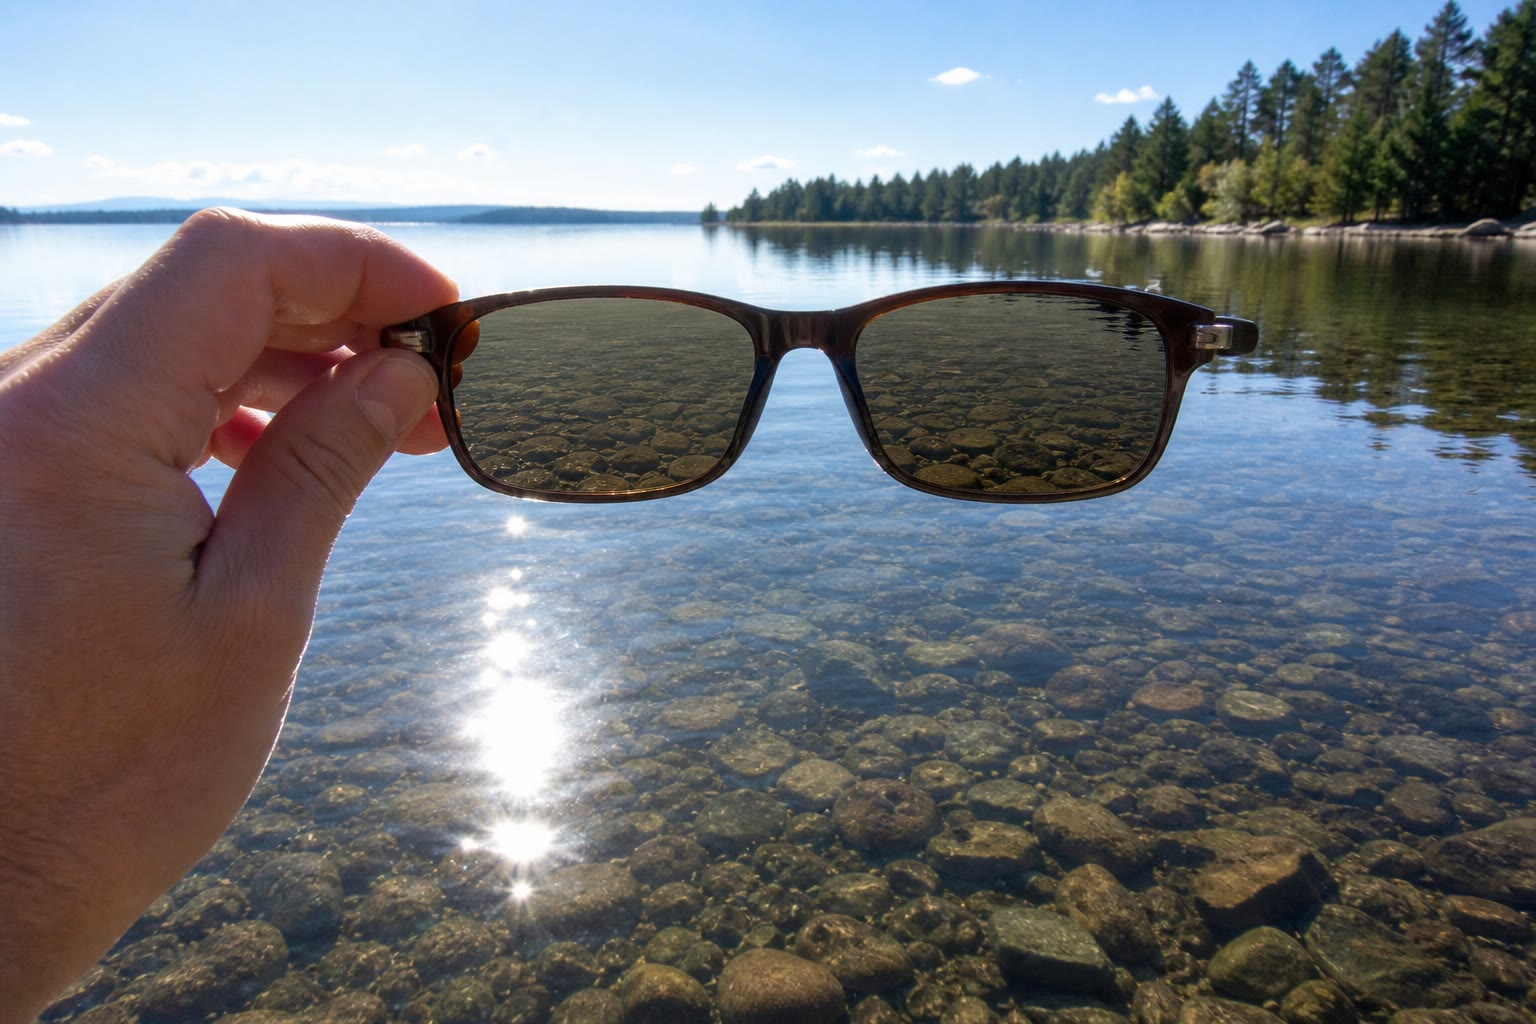
\includegraphics[width=0.58\linewidth]{images/book4/ai/b4-13-polarizing-sunglasses-lake.jpg}

{\small Óculos de sol polarizados diante de um lago: o brilho, refletido perto do ângulo de Brewster e polarizado horizontalmente, é cortado pelo eixo de transmissão vertical das lentes, e o fundo do lago aparece.}
\end{omfigure}

\section{Problema: A onda, a tela e a vela}

\begin{problem}[{Problema de fim de semana --- um feixe de laser desmontado em seus
campos, uma tela que pinta com polarização e uma sonda que
navega à luz}]
\label{pb:b2:plane-waves-polarization:1}

\medskip
\noindent\textbf{Parte I --- O feixe.}
Um laser de hélio--neônio emite \qty{10}{mW} a \qty{632.8}{nm} num feixe de
\qty{1.0}{mm} de diâmetro, polarizado retilineamente segundo $x$, viajando segundo
$z$.
\begin{enumerate}
  \item Frequência, número de onda, energia do fóton; fótons emitidos por
        segundo.
  \item Intensidade; amplitudes $E_0$ e $B_0$; escreva $\vect E(z, t)$ e
        $\vect B(z, t)$.
  \item Densidade de energia (média) e energia contida em \qty{1}{m} de
        feixe; que comprimento tem o feixe emitido em \qty{1}{ns}, e quantos
        comprimentos de onda ele contém?
  \item \omterm{thm:b2:poynting-vector:poynting}{Vetor de Poynting}: valor médio e sua oscilação; quantidade de movimento
        transportada por segundo; força sobre um alvo preto e sobre um espelho.
  \item Compare $E_0$ com o campo que liga o elétron num
        átomo de hidrogênio (\qty{5e11}{V/m}) e $B_0$ com o campo da Terra
        (\qty{50}{\micro T}).
  \item \omterm{prop:b2:poynting-vector:wave}{Pressão de radiação} sobre um anteparo preto, em pascals.
  \item Um elétron livre colocado no feixe: amplitude de sua oscilação
        de velocidade no campo elétrico (despreze primeiro a força
        magnética); razão entre a força magnética e a elétrica sobre ele ---
        por que a força magnética é desprezível para a matéria na luz
        comum?
  \item Escreva os campos do mesmo feixe se ele fosse polarizado
        circularmente; o que muda na intensidade, no \omterm{thm:b2:poynting-vector:poynting}{vetor de Poynting}
        e em sua dependência com o tempo?
  \item O feixe atravessa um polarizador cujo eixo faz
        \qty{30}{\degree} com $x$: potência transmitida; depois um segundo
        cruzado com o primeiro: potência; insira entre eles um
        terceiro a \qty{45}{\degree} do primeiro: potência.
\end{enumerate}

\medskip
\noindent\textbf{Parte II --- A tela.}
Uma tela de cristal líquido: retroiluminação (\omterm{def:b2:plane-waves-polarization:states}{luz natural}), um polarizador, a
célula e um polarizador cruzado. Sem tensão a célula gira a
polarização de \qty{90}{\degree}; com tensão ela não faz nada.
\begin{enumerate}[resume]
  \item Fração da intensidade da retroiluminação transmitida no
        estado claro (polarizadores perfeitos); e no estado escuro.
  \item Uma tensão intermediária faz a célula se comportar como um retardador
        de fase $\delta$ entre seus eixos, que estão a \qty{45}{\degree} dos
        polarizadores (sem rotação): mostre que a transmissão vale
        $\sin^2(\delta/2)$ --- a escala de cinzas.
  \item Vista através de um polarizador girado a \qty{90}{\degree} do
        polarizador de saída da tela, o que se vê? E a \qty{45}{\degree}?
  \item Uma \omterm{prop:b2:plane-waves-polarization:plates}{lâmina de quarto de onda} colada na tela a \qty{45}{\degree} de seu
        polarizador torna a saída circular: qual a vantagem para quem
        usa óculos de sol polarizados?
  \item Polarizadores perfeitos deixariam passar metade da retroiluminação no
        estado claro; folhas reais transmitem $85\%$ do ideal cada uma, e
        os filtros coloridos de um pixel deixam passar um terço da luz:
        fração da potência da retroiluminação que chega a quem olha, no branco;
        nomeie os dois lugares onde a maior parte da luz se perde.
  \item Folhas cruzadas reais vazam $0.1\%$ da luz: razão de contraste
        da tela (claro sobre escuro) numa sala escura.
  \item Os "polarizadores circulares" dos fotógrafos são um polarizador retilíneo
        seguido de uma \omterm{prop:b2:plane-waves-polarization:plates}{lâmina de quarto de onda} a \qty{45}{\degree}: o que a
        câmera recebe, e por que isso é melhor para o divisor de feixe
        sensível à polarização do seu autofoco do que
        luz retilínea?
  \item Por que os óculos de cinema 3D usam \omterm{def:b2:plane-waves-polarization:states}{polarização circular} em vez de
        retilínea? O que acontece com a diafonia entre os olhos
        se quem assiste inclina a cabeça de \qty{20}{\degree} com óculos
        retilíneos (intensidade que vaza para o olho errado)?
\end{enumerate}

\medskip
\noindent\textbf{Parte III --- A vela.}
Uma vela solar de área $S = \qty{1000}{m^2}$ e massa total $m = \qty{50}{kg}$,
perfeitamente refletora, a $D = \qty{1.0}{au} = \qty{1.5e11}{m}$ do Sol
($I = \qty{1.36}{kW/m^2}$; gravidade do Sol ali \qty{5.9e-3}{m/s^2}).
\begin{enumerate}[resume]
  \item Força de radiação quando a vela está de frente para o Sol; aceleração;
        razão em relação à gravidade solar.
  \item A vela é inclinada de $\theta$ em relação à posição de frente para o Sol: mostre que a
        força é normal à vela e proporcional a $\cos^2\theta$
        (potência interceptada $\times\cos\theta$, variação da quantidade de movimento segundo a
        normal $\times\cos\theta$).
  \item Para espiralar para fora, a vela mantém uma componente de força ao longo de sua
        velocidade orbital: para $\theta = \qty{35}{\degree}$, aceleração
        tangencial; celeridade ganha por ano; compare com a celeridade
        orbital da Terra (\qty{30}{km/s}).
  \item Por que a mesma vela, perto de Mercúrio ($D = \qty{0.39}{au}$), recebe
        $6.6$ vezes a força, e por que a razão em relação à gravidade
        não muda?
  \item O filme da vela tem \qty{2}{\micro m} de plástico aluminizado: sua
        temperatura ao sol se ela absorve $10\%$ e irradia pelas
        duas faces como um corpo negro ($\sigma = \qty{5.67e-8}{W.m^{-2}.K^{-4}}$).
  \item Tempo necessário para ganhar \qty{1}{km/s} de frente para o Sol; o que uma
        vela absorvedora (preta) do mesmo tamanho conseguiria?
  \item Confira a quantidade de movimento da luz com fótons: número de fótons
        que atingem a vela por segundo (\qty{2}{eV} em média) e a
        quantidade de movimento $hf/c$ de cada um; recupere a força.
  \item Faça o balanço: as três grandezas transportadas pela onda (energia,
        quantidade de movimento, polarização) e o dispositivo deste problema que
        explora cada uma.
\end{enumerate}
\end{problem}
